\documentclass[tikz,border=8pt]{standalone}
% Shared TikZ style for synorg platform diagrams. Each diagram \input's this
% inside a standalone document. Palette tracks the Material "teal" site theme so
% figures read as one system in light mode (SVGs are theme-neutral otherwise).
\usetikzlibrary{arrows.meta,positioning,shapes.geometric,fit,backgrounds,calc,decorations.pathreplacing}

\definecolor{synteal}{HTML}{00897B}   % primary
\definecolor{synfill}{HTML}{E0F2F1}   % light fill
\definecolor{synamber}{HTML}{B26A00}  % warning / lend
\definecolor{synred}{HTML}{B00020}    % deny / danger
\definecolor{syngrey}{HTML}{5F6368}   % muted

\tikzset{
  >=Stealth,
  font=\sffamily\small,
  box/.style={draw=synteal,line width=0.6pt,rounded corners=2pt,fill=synfill,
              inner sep=5pt,align=center},
  plane/.style={draw=synteal,line width=0.8pt,rounded corners=3pt,fill=synfill,
                inner sep=8pt,align=center},
  state/.style={draw=synteal,line width=0.7pt,circle,fill=synfill,inner sep=3pt,
                minimum size=11mm,align=center,font=\sffamily\footnotesize},
  decision/.style={draw=synteal,line width=0.7pt,diamond,aspect=2,fill=synfill,
                   inner sep=1pt,align=center,font=\sffamily\footnotesize},
  deny/.style={draw=synred,fill=synred!8,text=synred},
  warn/.style={draw=synamber,fill=synamber!10},
  flow/.style={->,line width=0.6pt,draw=syngrey},
  flowlbl/.style={font=\sffamily\footnotesize,text=syngrey,inner sep=2pt},
  note/.style={font=\sffamily\footnotesize\itshape,text=syngrey},
}

\begin{document}
% The preemption contract (training-onboarding.md, KTD12): checkpoint every <=5
% min; on preemption a 120 s grace flushes a final checkpoint; the job resumes on
% a fresh node from the last checkpoint, losing at most one interval (<=5 min).
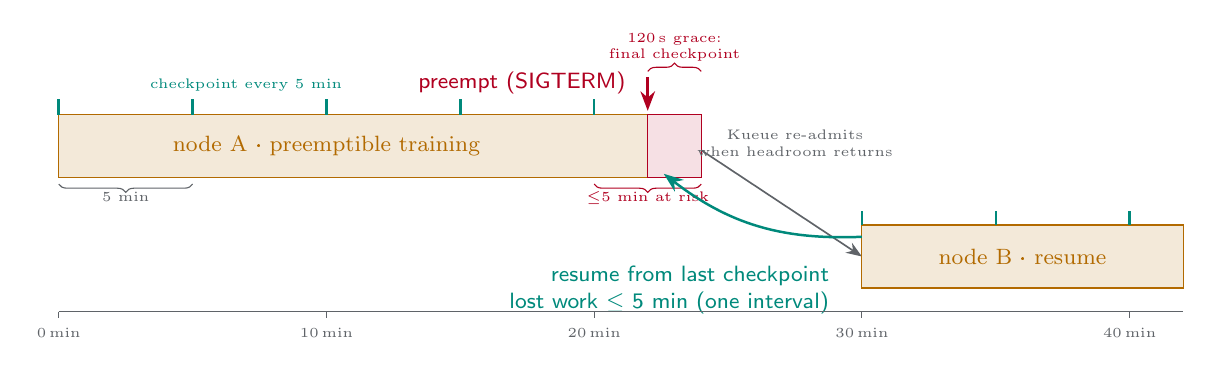
\begin{tikzpicture}[x=3.4mm,y=10mm]
  % ---- node A: the preempted run ----
  \draw[draw=synamber,fill=synamber!15] (0,0) rectangle (24,0.8);
  \draw[draw=synred,fill=synred!12]     (22,0) rectangle (24,0.8);
  \node[font=\footnotesize,text=synamber] at (10,0.4) {node A · preemptible training};

  % checkpoint ticks every 5 min
  \foreach \t in {0,5,10,15,20}{
    \draw[draw=synteal,line width=0.9pt] (\t,0.8) -- (\t,1.0);
  }
  \node[flowlbl,text=synteal,anchor=south,font=\tiny] at (7,1.02)
    {checkpoint every 5 min};
  % interval + at-risk braces below node A
  \draw[decorate,decoration={brace,amplitude=3pt,mirror},draw=syngrey]
    (0,-0.08) -- (5,-0.08);
  \node[flowlbl,font=\tiny,anchor=north] at (2.5,-0.1) {5 min};
  \draw[decorate,decoration={brace,amplitude=3pt,mirror},draw=synred]
    (20,-0.08) -- (24,-0.08);
  \node[flowlbl,text=synred,font=\tiny,anchor=north] at (22,-0.1) {$\le$5 min at risk};

  % preemption marker (label to the left of the line)
  \draw[flow,draw=synred,line width=0.9pt] (22,1.28) -- (22,0.85);
  \node[flowlbl,text=synred,anchor=east] at (21.4,1.2) {preempt (SIGTERM)};
  % 120 s grace brace above the red segment
  \draw[decorate,decoration={brace,amplitude=3pt},draw=synred] (22,1.35) -- (24,1.35);
  \node[flowlbl,text=synred,anchor=south,font=\tiny,align=center] at (23,1.4)
    {120\,s grace:\\final checkpoint};

  % ---- re-admission gap ----
  \draw[flow,draw=syngrey] (24,0.35) -- (30,-1.0);
  \node[note,font=\tiny,align=center,anchor=south] at (27.5,0.15)
    {Kueue re-admits\\when headroom returns};

  % ---- node B: resume on a fresh node ----
  \draw[draw=synamber,fill=synamber!15] (30,-1.4) rectangle (42,-0.6);
  \node[font=\footnotesize,text=synamber] at (36,-1.0) {node B · resume};
  \foreach \t in {30,35,40}{
    \draw[draw=synteal,line width=0.9pt] (\t,-0.6) -- (\t,-0.42);
  }

  % resume-from-last-checkpoint arc back into node A
  \draw[flow,draw=synteal,line width=0.9pt] (30,-0.75) to[bend left=20] (22.6,0.05);
  \node[flowlbl,text=synteal,anchor=north east,align=right] at (29,-1.05)
    {resume from last checkpoint\\lost work $\le$ 5 min (one interval)};

  % ---- time axis ----
  \draw[draw=syngrey,line width=0.5pt] (0,-1.7) -- (42,-1.7);
  \foreach \t in {0,10,20,30,40}{
    \draw[draw=syngrey] (\t,-1.7) -- (\t,-1.78);
    \node[font=\tiny,text=syngrey,anchor=north] at (\t,-1.78) {\t\,min};
  }
\end{tikzpicture}
\end{document}
